%
% latex-sample.tex
%
% This LaTeX source file provides a template for a typical research paper.
%

%
% Use the standard article template.
%
\documentclass{article}

\usepackage{geometry}
\geometry{letterpaper}

\usepackage{cite}
\usepackage{doc}
\usepackage{url}
\usepackage{graphicx}
\usepackage{aaai}
\usepackage{amsmath}
\usepackage{epstopdf}

\title{Energy Disaggregation}
\author{Henry Agsten, Jacob Denson, Jesse Huard, Isabel McCarten, Morgan Redshaw}
\date{}

\begin{document}

\maketitle

\begin{abstract}
Whatever we exactly did. Something about how, for Internet of Things, device on/off is more readily available
Would be very useful if could train off it combined with the aggregated data, rather than also using the disaggregated data or taking an unsupervised approach.
\end{abstract}

NOTE: Needs to be cleaned up now
NOTE: sub-metering is the word we want for measuring disaggregated energy signals
%TODO: Do we assume that are either ON or OFF, or that they can have multiple levels?
	%NOTE: another paper assumed that 'all appliances that have more than two states (e.g., on and off) will produce events that can be explained by two-state appliances'
%TODO: Outline where we got the data from

\section{Introduction}

Energy disaggregation, or non-intrusive load-monitoring (NILM), is the problem of estimating a household's individual appliance energy consumption given measurements from a single sensor which records the aggregate power consumption of the household over time.
While measuring the power draw of each device in a home directly yields more accurate results than machine learned techniques, it usually involves either expensive instrumentation of the devices we wish to measure the energy consumption of, or an intrusion into the home in order to set up power monitoring hardware.
Both situations are undesirable for the homeowner, so instead NILM makes use of already existing infrastructure combined with machine learned techniques, in order to provide an estimate of device energy consumption.

Having access to disaggregated energy consumption is useful to homeowners, as studies have shown that when presented with this information, they are more motivated to reduce their energy consumption \cite{Darby}.
Additionally, this information can be used to identify devices in a home which have become faulty and are in need of repair.
When a device breaks, changes in its energy consumption patterns can be detected by an automated system, allowing the homeowner to be notified that the device needs servicing.

Most existing machine learning methodologies for NILM are trained using data from households which have been instrumented to record the power consumption of each device separately, in addition to the aggregate household power usage \cite{Kelly, Cicchetti}.
However, as noted above, this instrumentation is expensive and makes it difficult to gather new data, with most existing datasets being limited to recording from only a small number of homes \cite{Redd}\cite{Kelly2}.
This lack of data from many homes has the effect of making it difficult to see how well current NILM algorithms generalize to unseen homes, and can be problematic with algorithms which require large amounts of data, such as deep neural network architectures \cite{Kelly}.


%TODO: Find paper that references difficulty of adapting to new house
**May not be correct** Due to the diversity of devices, both which are used in a house and their power consumption, it can be difficult to generalize from one house to another.

%TODO: List of a few papers that require this. Include all that we are referencing at other spots and that do this
Many existing methodologies for NILM require the aggregated energy usage for a house and the energy usage for each appliance of interest during the same time period \cite{Kelly, Cicchetti}. 
%TODO: Find paper that references this. Also, sentence should be better
However, recording the energy usage for each device is difficult, due to the requirement of adding sensors to each device.
With the increase in the Internet of Things, we expect that more devices will be able to indicate when they are using power to the server.
It is, however, unlikely that the necessary means to record the actual power usage will be installed into these devices.
Thus, the existing methodologies would not be able to benefit from these changes in devices.


%TODO: This needs to clearly outline that we are NOT learning on the specific house, to handle future data, but are instead preprocessing for the training data
In this report, we investigate different methods for taking the aggregated energy usage and information for when devices are on and generate information about how much power each device was using.


%TODO: What did we accomplish

\section{Related Work}

%NOTE: Should focus on research relevant to ours. Don't know how much there is.
%TODO: Should also outline one or two unsupervised approaches.
As far as we know, no studies of NILM using only information about the activity of each device per timestep, exist.
%TODO: Cite all of these
There have been supervised approaches using the disaggregated energy\cite{Kelly} or energy signatures \cite{Parson} for each device.
Some unsupervised approaches also exist that only use the aggregated energy of the overall house \cite{Kolter}.
%TODO: Mention something about related approaches or similar ideas?

%\subsection{Independent Component Analysis}

%TODO: Soundwaves is the wrong word
%To use ICA, we would need to assume that the signature for each device is statistically independent, which is unfortunately not true.
%TODO: Find citation for this
%As well, ICA performs best when there are multiple different 'sound waves', but with NILM there would only be the power being used by the house for each timestep.
%Thus, we believe that applying independent component analysis will not achieve significantly better results to existing methods.

%TODO: Should these be the approach name, or something else?

\subsection{Approaches using no information about single device consumption}
Unsupervised proceedings to disaggregate consumption data reliey mainly on Hidden Markov Models. 
Kolter \cite{Kolter} uses one Hidden Markov Model per device to describe its consumption and figure out at what time 
it was active. He finds periods of activity, clusters similar ones and builds a Hidden Markov Model per device. 
Unfortunately the proceeding to find these periods is not described in detail but seems to look for intervals when only 
one device is active, what we want to enhance. He states to reach precision values of over 90\% for some devices but since the recall values are not 
given it is harsh to judge these results. 
In contrast to this completely unsupervised approach Parson starts with knowledge about the general device type and 
offers for each device a generic model, which is fitted to the actual device. His biggest benefits are to identify the 
devices without labeling manually, since his generic models are labeled once and that he compares the house's device with 
the set of models, whereby it is not necessary to know how many device are in the house. For devices with clearly distinguish patterns 
(e.g. fridges) Parson reaches F-scores up to 85\% while achieving results under 20\% for unstable devices (e.g. Microwaves)
Even though his allocation of generic models and minute-wise measurements did not seem useful for us, his work leaded 
us to the used REDD-dataset 
and to the idea look for timesteps when only one device changes its activity status.
\subsection{Approaches using information about single device consumption}

%TODO: Citations for this
The most common supervised approaches use Hidden Markov Models as well as neural networks to estimate the power consumption 
for each device.

Well known is Parson's \cite{Parson} usage of one difference Hidden Markov Model (dHMM) per device to describe its 
consumption and figure out at what time it was active.
%TODO: Make sure is correct, and possibly cite this
A dHMM extends traditional Hidden-Markov-Models by additional hidden variables for the difference from the previous 
to current state. While this approach does not require the disaggreated energy signature per device, it does require 
prior knowledge in the form of ???

Latest progress was made by applying deep neural nets, where Kelly and Knottenbelt \cite{Kelly} used recurrent neural 
nets with four hidden layers and achieved positive results for stable-behaving devices, but lacked accuracy for multi-stated 
ones, leading to a F-score of 51\%. They also considered denoising autoencoders training one neural net per appliance. 
The neural net takes the power consumption within a sliding window as input and separates the devices consumption from 
the remaining power. Determining the window size by the usual activity time of the device they achieve an F-score of 70\%. 
Both of their approaches use in the training phase the separated energy consumption for every device, ignoring possible inherent 
relationships between different devices. Furthermore they identify that often signal reconstruction is not integral to applications.
Therefore, they take their task to be identification of a begin time, end time, and overall energy usage of a specific device, 
during the first cycle it is used.
%They attempt to solve the problem via an amalgamation of Constitutional, Feed forward, and recurrent neural nets, combined with 
%a denoising error\footnote{Viewing other data as `noise' may also cut out the holistic approach to the problem, removing the 
%problem of global consistency.} and training on each device individually\footnote{This may ignore inherent relationships between 
%different devices (though perhaps the neural networks account for this).
%Perhaps a way to `double check' nets are correct may provide a more effective, holistic approach.}.
%Due to the extensive data set one needs to train deep nets, the pair generates synthetic data by combining data with `noise' data\footnote{The data they generate is naive, and we will likely see performance increases from a more realistic generation of data, or through pre-training on large amounts of unlabelled data, then a less extensive training on real data.}.
Weiss \cite{Weiss} presumes the power consumption as a sequence of piecewise constant consumption levels those differences 
describe the typical consumption pattern of a distinct device. They identify devices by checking for characteristic 
differences 
between consumption changes and look for the most similar device pattern via neareast neighbor calculation. Since they get remarkable 
F-scores of 80\% and higher for some devices although the strong assumption we also have a look on signal for which this assumption holds.


%I did not understand how data was selected for training, but I do no it is normalized to have mean zero -- which may or may not reduce the ability to consistently identify features.
​
%Questions about the paper:
%
%\begin{enumerate}
%	\item Using Convolutional Neural networks (Time Invariant).
%	\item Ignoring all but first activation.
%	\item Why does the algorithm ignore all but the first activation.
%	\item Local to Global.
%	\item NILMTK will be useful!
%	\item Periodicity.
%\end{enumerate}
​
%One neural network is trained per target appliance, based on real data and synthetically generated data.

%**Another interesting aspect of the paper was how they used Denoising Autoencoders.
​
\subsubsection{Deep Recurrent Neural Networks}
​
A standard recurrent neural network with $t$ layers assumes a statistical model is parameterized by matrices $A,B$ and $C$ and a bias vector $b$, where if $x = (x_1, \dots, x_n)$ is observed, then our output $y$ is generated iteratively by the equations
%
\[ h_t = \sigma(A h_{t-1} + B x + b) \]
%
\[ y = C h_N \]
%
We feed our data through the neural network $N$ times before generating the output.
It may be of interest to use Long short-term memory architectures, defining $h_t$ instead by
%
\[ I_t = \sigma(Ax + B h_{t-1} + C c_{t-1} + b_1) \]
%
\[ F_t = \sigma(Dx + E h_{t-1} + F c_{t-1} + b_2) \]
%
\[ c_t = F_t c_{t-1} + I_t \tanh(G x + H h_{t-1} + b_3) \]
%
\[ o_t = \sigma(K x + L h + M c_t + b_4) \]
%
\[ h_t = o_t \tanh(c_t) \]
​
Bidirectional networks use forward and backward sequences, which compute ...
​
What's nice about these types of neural networks is that we can analyze them as a dynamical system -- which matches up nicely as viewing pre-training as a dynamical system!

Used in \cite{Kelly}.

\subsubsection{Baranski's Algorithm}

\subsubsection{Denoising Autoencoders}

Again, used in \cite{Kelly}.
%TODO: What is good/bad about them



\section{Our Stuff}

%TODO: This one could be useful
%Known as nonintrusive load monitoring (NILM) various researchers have investigated this problem.
%Weiss (Source3?) presume the power consumption as a sequence of piecewise constant consumption levels whose differences describe the typical consumption pattern of a distinct device.
%Since they get remarkable F-scores of 80\% and higher for some devices we also had a look for signal where this assumption holds.

Unlike many of the other methods, we are assuming that we do not have the disaggregated power signature for each device during the learning stage.
Instead, we assume to instead have accurate information about when each device is active, due to the trend of the "Internet of Things".
Where many devices are connected to the internet, and could thus provide information about when they are active.
%TODO: Get paper for this?


\subsection{Dataset}
As a basis to evaluate our approach we use the Reference Energy Disaggregation Data Set (REDD) \cite{Redd}, a collection of energy consumption 
from six houses where the mains, single devices and circuits were measured separately over two weeks. Even though the data set contains high-frequent 
measurings we use the ones with frequencies between $1$ and $3 Hz$, to stay comparable to former works with similar frequencies. Since not all 
device exist in every house we focused on the most common ones: dishwasher, washer-dryer-combinations (both in all houses), refridgerator (in 5 
out of 6 houses) as well as microwave and stove (in all but two houses). Since the sum of all single devices and circuits does not sum up to the 
measured overall consumption, because small devices like consumer electronics were not traced, we compare two different approaches one with noise 
and one without. For the unnoised method we sum up only the consumption of the focused devices and take their sum as the aggregated energy consumption. 
We check these results against the ones where we subtract the devices which are not of interest for us from the measured overall consumption, which 
gives us a bigger than natural noise.\\
Our goal is to work only with the information if a device is inactive or active, whereby active means that it is actually on and not only in a
standby mode. To generate the  on/off-indicators we check the dataset against a threshold $\delta$, assigning the device an indicator of $1$ if its 
consumption in the regarding time step exceeds the threshhold and considering the device as inactive otherwise, assigning $0$. Using the threshold 
eliminates the uninteresting phases of permant standby uses, as they are common especially in refridgerators.

\section{Preprocessing}
​
Robust evaluation metrics are essential to applying supervised learning techniques. Unfortunately, obtaining reasonable metrics is near impossible without actual power outputs of individual devices. Nonetheless, we are still interested in applying supervised approaches, which have a strong history of success in energy disaggregation. Our solution estimates individual outputs on the training data, as a preprocessing step to train a more powerful prediction algorithm. We emphasize that as a general prediction method, the preprocessing algorithms we describe are not viable, since after the training phase we have no access to device on/off indicators, which are key in obtaining power output.
​
Inferring general power outputs is an underdetermined problem. Good results can therefore only be obtained by making strict assumptions about the statistical model producing the data. Here, we apply two separate models: The simplest assumes that good estimates are obtained from a constant power estimate, the second that each device is represented by a restricted family of markov processes.
​
In the sequel, the following notation will be convinient. We shall let $N$ denote the number of devices we are observing, and $T$ the number of time epochs. The random variable $X_i^t$ models the output of the device $i$ at the time $t$, and $Y^t = \sum X_i^t$ denotes the total power output. We observe the indicators $I_i^t = \mathbf{I}(X_i^t > 0)$ and $Y^t$ over the range of $i$ and $t$, and must predict the $X_i^t$ to the best of our ability.
​
\subsection{A Constant Power Assumption}
​
In our first model, we assume that the output of devices are mutually independant, and that the outputs of a specific device are i.i.d with respect to time, when that device is switched on. The mathematics tells us that there are numbers $P_1, \dots, P_n \in \mathbf{R}^+$ for which $X_i^t = P_i + \varepsilon_i$, where $\mathbf{E}(\varepsilon_i) = 0$. Assuming error variances are small, we conclude that treating the power output of a device as constant when it is switched on is accurate, and our problem reduces to finding the values $P_i$. After the $P_i$ are predicted, output estimations are calculated
%
\[ \hat{X_i^t} = I_i^t P_i \]
%
Finding $P_i$ is feasable, once an optimization metric is obtained.
​
The simplest way to choose the $P_i$ is to minimize the $L_2$ error of our estimated total
%
\[ \hat{Y}^t = \sum_{i = 1}^n \hat{X_i^t} = \sum_{i = 1}^n I_i^t P_i \]
%
with respect to the known total $Y^t$. This leads to thehis can be easily found by the optimization
%
\[ \min_{P_1, \dots, P_n \in \mathbf{R}^+} \sum_{t = 1}^T \left( Y^t - \sum_{i = 1}^n I_i^t P_i \right)^2 \]
%
In our implementation, we use Scipy's {\it optimize()} method to determine the $P_i$, which uses one of a range of non-linear optimization algorithms.
​
\subsection{Estimating Difference Markov Processes}
​
An alternate model assumes the underlying processes generating appliance power outputs are mutually independant markov models. As an extension of the previous model, the power outputs of devices are constant when the underlying chain remains in a single state. This should suffice for most practical applications, since most appliances change their power load only when running in a different `mode' (an oven cooking at different temperatures, a computer under different stress levels, etc.).
​
Mathematically speaking, the outputs $X_i^t$ are drawn from some hidden markov model with states $S^i_0, S^i_1, \dots, S^i_{K_i}$, where $S_0$ is the `off' state ($X_i^t = 0$) and that, given that the markov model is in a state $S^i_k$ at some time $t$, then $X_i^t \sim \mu_i^k + \varepsilon_i^k$, where $\mathbf{E}(\varepsilon_i) = 0$, and $\mu_i^k \in \mathbf{R}^+$ are fixed. Once we have estimated such a model, we may estimate the $X_i^t$ by a best fit method -- calculating the state transition that results in the best fit. We don't ever need to calculate transition probabilities, since our knowledge of the indicator functions effectively removes most of the randomness from the calculation.
​
Hidden markov chains are still difficult to estimate, so restriction of the markov model's structure is necessary. In words, we restrict the model such that it is unable to transition from any on state to any on state directly -- it must pass through the off state in order to transition to these states. A general diagram for such a markov chain is displayed below. It is hard enough to estimate the means, so we assume that the states of the markov diagram have been given by divine insight -- this is a classic problem; too many states will overfit the data, too few will underfit.
%
% PLACEHOLDER IMAGE
\begin{center}
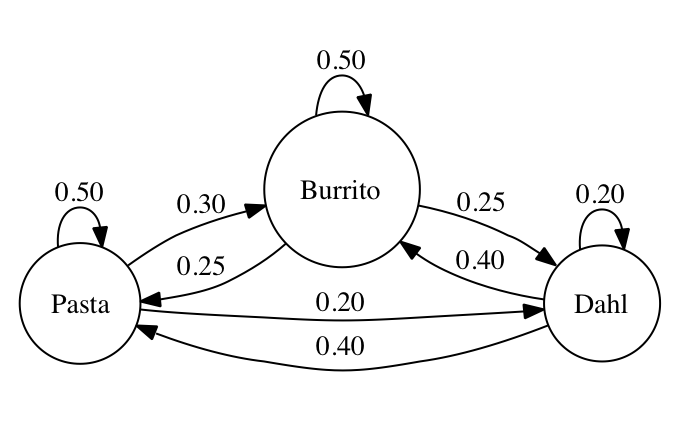
\includegraphics[scale = 0.5]{process-probabilities}
\end{center}
%
To further reduce the dimensionality, we follow Kolter's approach to the Markov model problem by considering difference Markov models\footnote{described in [1], see the section on additive markov models}. Rather than working with the data $Y^t$, we choose only to use values $\Delta Y^t := Y^t - Y^{t-1}$ at timepoints $t$ where the $i$'th device switches on ($\mathbf{I}(X_i^{t-1} > 0) = 0$ and $\mathbf{I}(X_i^t > 0) = 1$). Hopefully, this difference describes the average power over the entire interval where the device is switched on. Even if it doesn't, we should have enough data to filter out errors. At these time points, it is very likely that our device will be the only device to change state, for we are effectively viewing a discrete embedding into a continuous time markov chain, and it is common knowledge that in such a chain that, given our embedding is sufficiently fine, two state changes will very rarely occur at once. We then attempt to optimize our choice of $\mu_i$ redefining $X_i^{t + k} = \Delta Y^t$, where $X_i^{t + l} > 0$ for $l \in \{0, 1, \dots, k\}$.
​
Now we shall describe the optimization for a specific device $i$. Suppose that, the device enters a series of intervals of lengths $l_1, \dots, l_M$, taking difference values $\Delta Y^{t_1}, \dots, \Delta Y^{t_M}$ in each interval. We proceed to determine the values $\mu_1, \dots, \mu_K$ by minimizing the best fit over the data. Minimization over the $L_1$ norm will be used, since we may take advantage of its discrete qualities
%
\begin{equation} \min_{\mu_1, \dots, \mu_K} \sum_{i = 1}^M l_i \min_{k \in \{ 1, \dots, K \}}|\Delta Y^{t_i} - \mu_k| \end{equation}
%
There is a geometric interpretations of this minimization. Viewing the $\Delta Y^{t_i}$ as points, each with a `weight' $l_i$, we are attempting to choose the best centers of mass $\mu_1, \dots \mu_n$ which distribute themselves evenly between the points $\Delta Y^{t_i}$.
​
If we vary just one of the means $\mu_i$ in (1), we obtain a piecewise linear function. It follows that the minima $\mu_i$ may always be chosen to lie at the edge points of the function, which are the values $\Delta Y^{t_i}$. This leads to a discrete problem (which is not true for other $L_p$ norms), which we may solve through dynamic programming. First, we order the $\Delta Y^{t_i}$. Suppose $\mu_1 < \mu_2 < \dots < \mu_K$ is the optimal solution to our problem. If we remove $\mu_K$, then $\mu_1 < \dots < \mu_{K-1}$ is the optimal solution to the subproblem of distributing $K-1$ means among the subset of points who's closest mean is not $\mu_K$ (for otherwise we can move these means to improve our current solution). We therefore can work backwards dynamically to obtain a solution. From this optimal substructure, we obtain the simple recurrence: If we let $L(m,k)$ be the optimum cost of putting $k$ of the $\mu_i$ in the range $\{ t_1, \dots, t_m \}$, then we may choose an interval $\{ t_p, \dots, t_m \}$ for which $\mu_k$ will be the closest estimate, and then we optimize over $\{ t_1, \dots, t_p \}$ with one less estimate. Our reccurence is
%
\begin{align*}
    L(m,k) = \min_{k \leq p < m} \bigg\{ L(p,k-1) + \min_{p < i \leq m} \sum_{j = p+1}^m l_j |Y^{t_j} - Y^{t_i}| \bigg\}
\end{align*}
%
\[ L(1,1) = 0 \]
%
By keeping track of the location of the means recursively, we can build up the optimal $\mu_i$.

\subsection{Task}



\subsection{Evaluation}
To compare our methods with each other and with existing approaches, we focus on two questions.\\
1. How well did we identify what devices where active in each time step?\\
2. How well did we identify the single devices‘ consumption?\\
To address the first question we use the F1-Score, ensuring our results to be comparable to the works in the section \textit{Literature}. The 
advantages of the F1-Score to combine recall and precision avoids contortions, which would arise by considering only one of them. Assume we 
identify the refridgerator being active in all time steps we get a optimal recall value, but a low precision, whereas we get a optimal precision 
by identifying the refridgerator never as active.
\[ \textrm{Precision} = \frac{\textrm{Number of true positive elements}}{\textrm{Number of elements identified as positives}}  \]
\[ \textrm{Recall} = \frac{\textrm{Number of true positives}}{\textrm{Number of elements that are indeed positive}}  \]
\[ \textrm{F1-Score} = \frac{2 \cdot \textrm{Precision} \cdot \textrm{Recall}}{\textrm{Precision} + \textrm{Recall}}\]
For the second question we are interested in the error per timestep and to generate acuuracy-like value. Therefore we
compare the disaggregated energy consumptions per device with the actual device's consumption we have from the REDD
dataset. Following \cite{Redd} we can compute the accuracy depending on the summed absolute deviation in relation to 
the overall consumption:
\[\textrm{Accuracy}_{abs} = 1- \frac{\sum^{T}_{t=1}\sum^{N}_{n=1}|\hat{y}^{(n)}_t-y^{(n)}_t|}{2 \sum^{T}_{t=1}Y_t} .  \]
The error per timestep can be similarly described as the absolute squared error:
\[\textrm{ASE} = \frac{\sum^{T}_{t=1}\sum^{N}_{n=1}|\hat{y}^{(n)}_t-y^{(n)}_t|}{T \cdot n} .  \]
While the absolute error weights all differences regardless of their size the same, we also want information about the accuracy when 
weighting bigger deviations higher than smaller ones. We use the root squared error instead of the squared error 
to stay within the same unit. Therewith we calculate the root mean squared error as the error per timestep and similar a respective 
accuracy as the ratio with summed up overall consumption.
\[\textrm{RMSE} = \sqrt{\frac{\sum^{T}_{t=1}\sum^{N}_{n=1}(\hat{y}^{(n)}_t-y^{(n)}_t)^2}{T \cdot n}} .  \]
\[\textrm{Accuracy}_{rse} = 1- \frac{\sqrt{\sum^{T}_{t=1}\sum^{N}_{n=1}(\hat{y}^{(n)}_t-y^{(n)}_t)^2}}{2 \sum^{T}_{t=1}Y_t} .  \]




%TODO: Whatever evaluation function to see how well the neural network does after training.
%May even want to use two or more, to see if they work better in different circumstances

%Then, we will compare the results for the different trained denoising autoencoder neural nets, based on the data that we preprocessed.

%Will train and evaluate on the devices %TODO: write out devices


%TODO: Example?



%TODO: Example?

\section{Discussion}

\subsection{Future work and Extension}

Extension to Baranski's Algorithm?.

HMM depending on how well that goes

% Generate the bibliography.

\bibliography{biblio}
\bibliographystyle{aaai}

\end{document}
